\documentclass[11pt]{article}
\newcommand{\name}{Jingbo Wang}

\usepackage[paper=letterpaper, margin=1in, headheight=13.6pt]{geometry}
\usepackage{fancyhdr}
\usepackage{booktabs}
\pagestyle{fancy}
\fancyhf{}
\rhead{\name{}}
\cfoot{Page \thepage}

\usepackage[parfill]{parskip}
\usepackage{amsmath}
\usepackage{graphicx}
\usepackage{fancyvrb}
\usepackage{upquote}

\begin{document}
\thispagestyle{empty}

\begin{center}
{\large CS 310}\\
Assignment 322\\
\today
\end{center}

\begin{flushright}
\name{}
\end{flushright}

The \texttt{avl.h} algorithm given in the assignment could build an "almost" 
balanced binary search tree. This is accomplished by \texttt{avl.h}.

The input size of the \texttt{avl.h} algorithm is \texttt{n}, the result \texttt{Y}
is the height of AVL Tree.

In my main function I use \texttt{default\_random\_engine} to get random number from 
0 -- \texttt{n} (\texttt{n} is my input size) and push this value by the function 
\texttt{insert} to get the AVL tree.

In the function \texttt{void insert(const Comparable\& data, AVL\_node*\& t)}:
\begin{Verbatim}[numbers=left,xleftmargin=5mm]
    if (t == nullptr)
    {
      t = new AVL_node(data, nullptr, nullptr);
    }
    else if (data < t->data)
    {
      insert(data, t->left);
      ...
    }
    else if (t->data < data)
    {
      insert(data, t->right);
      ...
    }
    t->height = std::max(height(t->left), height(t->right)) + 1;
\end{Verbatim}

In function \texttt{insert}, we use recursion to find where we could insert the data 
in the AVL tree. If \texttt{data} is smaller than \texttt{t->data}, so \texttt{data} 
goes \texttt{insert(data, t->left)} in Line 7, so does for \texttt{insert(data, t->right)}
in Line 12, until it finds that \texttt{t} is \texttt{nullptr}, we a new \texttt{AVL\_node}
and insert \texttt{data} here. When the \texttt{insert} function calls, it always runs
Line 15, to get each height of the node \texttt{t} that roots the subtree.

After insert \texttt{data}, function will test the height-balanced of the node \texttt{t} 
that roots the subtree beginning with \texttt{data}'s parent until to the top that roots 
the AVL tree. if \texttt{t}'s height-balanced is equals to 2, it will run \texttt{RR}, 
\texttt{RL}, \texttt{LL} and \texttt{LR} functions in lines 8, and 13 which I don't quote 
in the sample to make binary search tree "almost" balance. 

For function \texttt{rotateRR}:
\begin{Verbatim}[numbers=left,xleftmargin=5mm]
void rotateRR(AVL_node*& p)
  {
    AVL_node* orig_right = p->right;
    p->right = orig_right->left;
    orig_right->left = p;
    p->height = std::max(height(p->right), height(p->left)) + 1;
    orig_right->height = std::max(height(orig_right->right), p->height) + 1;
    p = orig_right;
  }
\end{Verbatim}
It runs when the height-balanced of node \texttt{p} is equal to 2, and \texttt{data}
is larger than \texttt{P->right->data}. In other words, when the new unbalancing node 
is at right of the AVL tree, we will use function RR that is rebalanced with 
rotating left to make it into a new balance ( height-balanced $<$ 2). 

So does function \texttt{LL} do, it is rebalanced with rotating right to make it into
a new balance. Also, it always runs when the new unbalancing node is at left of 
the AVL tree.

For function \texttt{RL}:
\begin{Verbatim}[numbers=left,xleftmargin=5mm]
void rotateRL(AVL_node*& p)
  {
    AVL_node *temp_p = p;
    rotateLL(temp_p->right);
    rotateRR(p);
  }
\end{Verbatim}
Function \texttt{rotateRL} runs function \texttt{LL} first at the right of \texttt{p}
, and then it runs function \texttt{RR} to make the whole tree being balance again. 

The situation of function \texttt{LR} is the opposite. It runs function \texttt{RR} at 
the left of \texttt{p} first and then it is function \texttt{LL}, so it could make 
the tree into balance again. 

After running all rotate functions, all nodes' height-balanced in the AVL tree are less 
than 2. In other words, every root and its leave are almost evenly distributed.

After runs with different input size:
\begin{Verbatim}
for n in $(seq 100 10 10000)
do
    ./program $n
    ./program $n
    ./program $n
done 2> results.dat
\end{Verbatim}

So, we could get:
\texttt{n} is input size, \texttt{Y} is the height of AVL tree.
\begin{table}[htbp]
    \centering
    \begin{tabular}{c|c}
        n & Y \\
    \hline
        1 & 1  \\
        2 & 2  \\
        3 & 2  \\
        4 & 3  \\
        5 & 3  \\
      100 & 8  \\
     1000 & 12  \\
    10000 & 16  \\ 
    \end{tabular}
    \caption{the height of AVL tree and input size relationship}
    \label{sum&n}
\end{table}

Thus, 
\begin{align*}
    Y &\leq 1.5\lg n \\
      &\in \Omega(\lg n)
\end{align*}     


in order to generate a set of points.  The resulting data were
plotted, giving the following.  Also plotted on the same axes are the
scaled standard functions $1.5\lg n$ which illustrate above the 
\texttt{AVL Tree Height} is worst case.

\begin{center}
  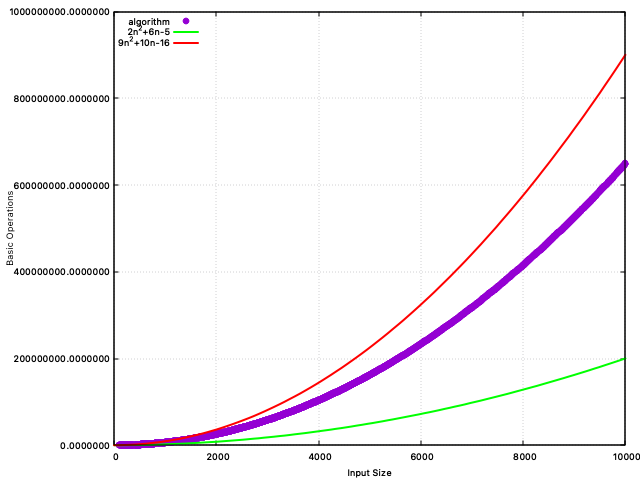
\includegraphics[width=0.7\textwidth]{analysis.png}
\end{center} 

We see that the plot confirms the theoretical analysis above. It is same
as we told in class.
\end{document}